\chapter{Theoretische Grundlagen}
\label{cha:theorie}

\section{Datenschutz und Datensicherheit in der öffentlichen Verwaltung}
\label{sec:datenschutz-verwaltung}
\begin{spacing}{1.5}

Datenschutz und Datensicherheit sind zentrale Aspekte bei der Verarbeitung personenbezogener Daten, insbesondere in der öffentlichen Verwaltung. Der Datenschutz basiert auf einer Reihe von Prinzipien, die sicherstellen sollen, dass personenbezogene Daten verantwortungsvoll und unter Wahrung der Rechte der betroffenen Personen verarbeitet werden. Zu diesen Prinzipien gehören unter anderem die Zweckbindung sowie die Datensparsamkeit bzw. Datenminimierung. Zweckbindung bedeutet, dass personenbezogene Daten nur für festgelegte, eindeutige und legitime Zwecke erhoben werden dürfen und nicht in einer mit diesen Zwecken unvereinbaren Weise weiterverarbeitet werden dürfen\footnote{gemäß Art. 5 Abs. 1 Buchst. b \acrshort{dsgvo}}. Datensparsamkeit bzw. -minimierung verlangt, dass nur so viele Daten wie nötig und nur die für den jeweiligen Zweck erforderlichen Informationen erhoben und verarbeitet werden\footnote{gemäß Art. 5 Abs. 1 Buchst. c \acrshort{dsgvo}}.

%\subsection*{Rechtliche Rahmenbedingungen}
Die \acrshort{dsgvo} ist das zentrale Gesetzeswerk zum Datenschutz in der Europäischen Union und legt strenge Regeln für die Verarbeitung personenbezogener Daten fest. Die \acrshort{dsgvo} gilt auch für die öffentliche Verwaltung und fordert, dass diese Einrichtungen geeignete technische und organisatorische Maßnahmen treffen, um den Schutz personenbezogener Daten zu gewährleisten\footnote{gemäß Art. 32 Abs. 1 \acrshort{dsgvo}}. Zusätzlich zur \acrshort{dsgvo} gibt es nationale Datenschutzgesetze, wie das Bundesdatenschutzgesetz (\acrshort{bdsg}) in Deutschland, die spezifische Regelungen für die öffentliche Verwaltung enthalten. So verpflichtet etwa das \acrshort{bdsg} öffentliche Stellen, so wenig personenbezogene Daten wie möglich zu verarbeiten und diese frühestmöglich zu anonymisieren oder zu pseudonymisieren\footnote{gemäß Art. 71 Abs. 1 \acrshort{bdsg}}.

%\subsection*{Besondere Herausforderungen in der öffentlichen Verwaltung}
Die öffentliche Verwaltung verarbeitet eine Vielzahl sensibler personenbezogener Daten\footnote{im Sinne von Art. 9 \acrshort{dsgvo}}, darunter biometrische Daten, Gesundheitsdaten und Daten im Zusammenhang mit Sozialleistungen. Diese Daten sind besonders schützenswert und erfordern daher erhöhte Sicherheitsmaßnahmen. Zudem sind öffentliche Verwaltungseinheiten oft dezentral organisiert, was zu Herausforderungen bei der Koordination und Umsetzung einheitlicher Datenschutzmaßnahmen führen kann. Transparenz und Rechenschaftspflicht sind weitere wichtige Aspekte, da öffentliche Einrichtungen gegenüber Bürgern und Aufsichtsbehörden verpflichtet sind, ihre Datenverarbeitung offen und nachvollziehbar zu gestalten\footnote{gemäß Art. 5 Abs. 1 Buchst. a \acrshort{dsgvo} und Art. 5 Abs. 2 \acrshort{dsgvo}}.

%\subsection*{Anonymisierung vs. Pseudonymisierung}
Ein wesentliches Element des Datenschutzes sind die Techniken der Anonymisierung und Pseudonymisierung. Pseudonymisierung ist der Prozess, bei dem Identifikationsmerkmale (z. B. Name und Adresse) durch Pseudonyme ersetzt werden, mit dem Ziel, die Re-Identifizierung zu erschweren. Der Begriff Anonymisierung beschreibt demgegenüber einen Prozess, bei dem personenbezogene Daten in einer Weise verändert werden, die eine Zuordnung zu einer bestimmten Person durch Dritte unmöglich macht oder aber mit einem unverhältnismäßig hohen Aufwand verbunden wäre\footnote{vgl. Art. 3 Abs. 6 \acrshort{bdsg} i.d.F.v. 2009}. Dies kann beispielsweise durch das Entfernen oder Verändern von Identifikatoren wie Namen und Adressen erreicht werden. Sie sind damit von den Beschränkungen der \acrshort{dsgvo} befreit \cite[184]{dewes_verfahren_2022}. Während bei der Pseudonymisierung eine Re-Identifizierung unter Zuhilfenahme gesondert aufbewahrter Zusatzinformationen möglich ist\footnote{gemäß Art. 4 Nr. 5 \acrshort{dsgvo}}, ist dies bei anonymisierten Daten praktisch ausgeschlossen. Gleichzeitig sinkt mit der Anonymisierung jedoch meist auch der Informationsgehalt und damit einhergehend die analytische Nutzbarkeit der Daten, da wichtige Zusammenhänge und Muster möglicherweise nicht mehr erkennbar sind.

\end{spacing}
\section{Grundlagen von Synthetic Data}
\label{sec:grundlagen-synthetic-data}
\begin{spacing}{1.5}

Synthetische Daten sind künstlich generierte Daten, die reale Daten nachahmen, ohne tatsächlich auf echte personenbezogene Informationen zurückzugreifen. Diese Daten werden durch algorithmische Prozesse erzeugt und sind darauf ausgelegt, die statistischen Eigenschaften und Strukturen echter Daten zu reproduzieren \cite[15]{hradec_multipurpose_2022}. Der Hauptzweck synthetischer Daten besteht darin, die gleichen Analysen und Anwendungen zu ermöglichen wie mit echten Daten, jedoch ohne die damit verbundenen Datenschutzrisiken. Sie bieten eine Möglichkeit, reale Daten zu ersetzen, wenn diese aufgrund von Datenschutzbestimmungen oder anderen Restriktionen nicht genutzt werden können.

Es gibt verschiedene Techniken zur Erzeugung synthetischer Daten, die je nach Anwendungsfall und erforderlicher Datenstruktur gewählt werden können. Eine der einfachsten Methoden ist das Random Sampling, bei dem Datenpunkte basierend auf den Wahrscheinlichkeitsverteilungen der Originaldaten generiert werden. Probabilistische Ansätze wie Markowmodelle \cite{saadi_hidden_markov_2016, huertas_generating_2018, dahmen_synsys_2019} und Bayes'sche Netze \cite{young_using_2009, kaur_application_2020, gogoshin_synthetic_2021} ermöglichen die Generierung neuer Kombinationen von Merkmalen, die in den ursprünglichen Daten nicht vorhanden sind. Mit der gestiegenen Rechenleistung haben Deep Generative Models (\acrshort{dgm}s), die Deep Learning für die Erstellung synthetischer Daten nutzen, stark an Bedeutung gewonnen. Zu den wichtigsten Modellen gehören Variational AutoEncoders (\acrshort{vae}s), die die Wahrscheinlichkeitsverteilung der Daten explizit formulieren, und Generative Adversarial Networks (\acrshort{gan}s), bei denen ein Generator realistisch aussehende Daten erstellt und ein Diskriminator diese als echt oder gefälscht einstuft (vgl. Abbildung \ref{fig:gan-architecture}) \cite[14]{hradec_multipurpose_2022}. Das endgültige Ziel besteht darin, ein Gleichgewicht zu erreichen, bei dem die generierten Daten der gleichen Verteilung folgen wie die realen Daten \cite[32]{jordon_synthetic_2022}. \acrshort{gan}s sind besonders erfolgreich, da sie keine gelabelten Daten benötigen und in vielen Bereichen, wie der Generierung von fotorealistischen Bildern, herausragende Ergebnisse erzielen \cite[7]{shrivastava_learning_2017}.

\newpage

\begin{figure}[ht]
\begin{center}
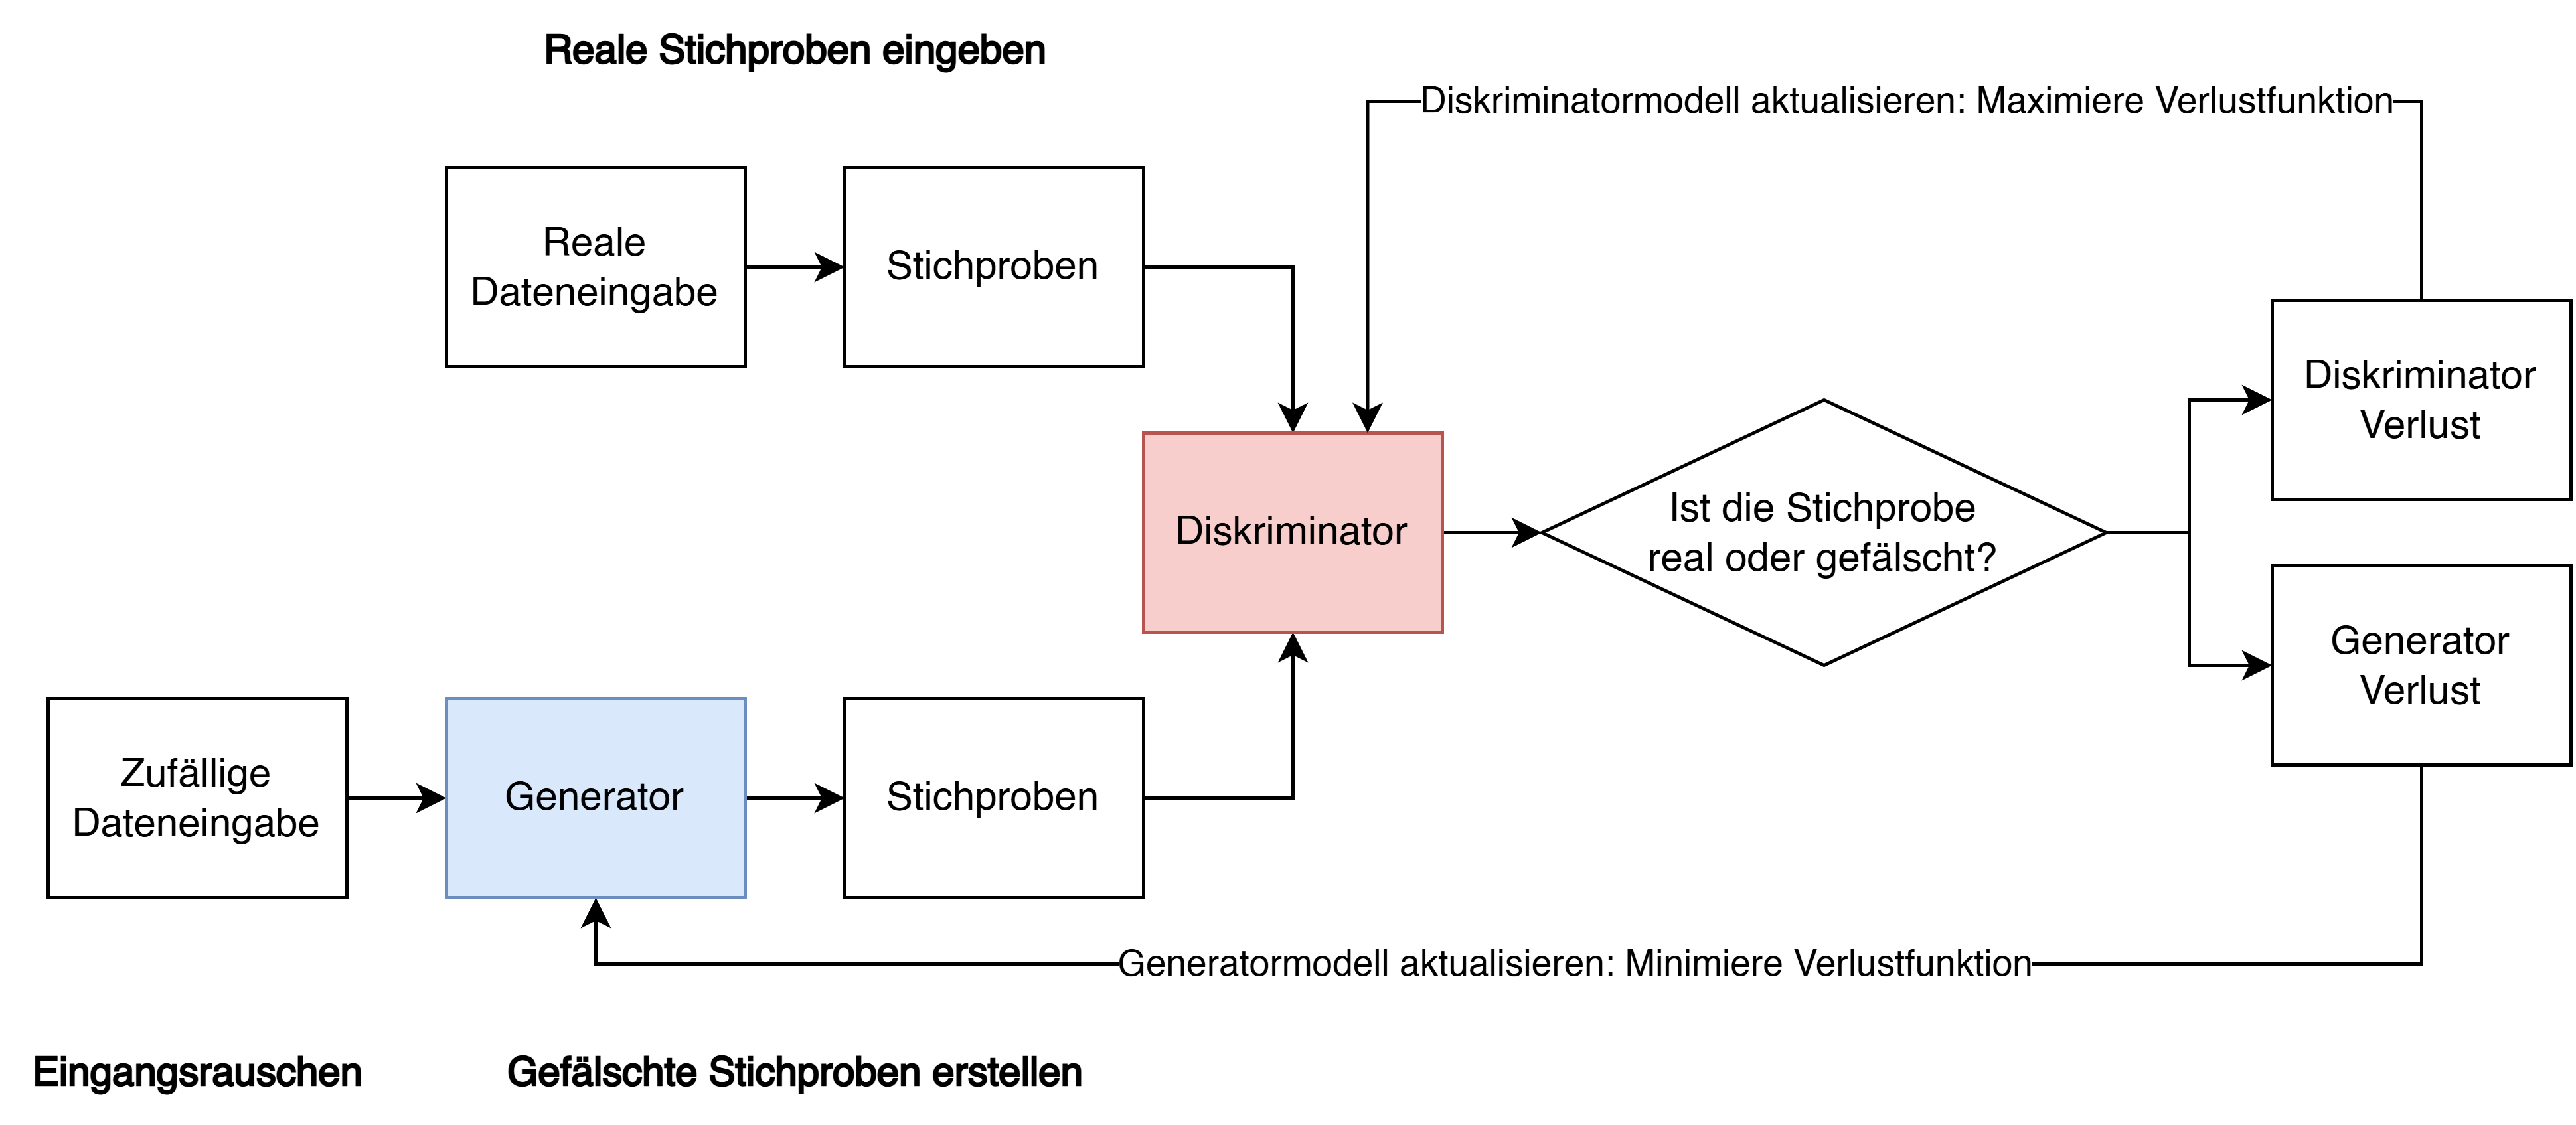
\includegraphics[width=\textwidth]{img/gan.png}
\caption[Architektur von Generative Adversarial Networks]{Architektur von Generative Adversarial Networks\footnotemark}
\label{fig:gan-architecture}
\end{center}
\end{figure}
\footnotetext{Eigene Darstellung in Anlehnung an \cite[672]{ramzan_generative_2024}}

Synthetische Daten finden in vielen Bereichen Anwendung. In der Forschung und Entwicklung bieten sie Daten für die Entwicklung und das Testen neuer Algorithmen und Modelle, ohne Datenschutzbestimmungen zu verletzen. In der Bildung und im Training können sie in Schulungen und Kursen verwendet werden, um realistische Datensätze zur Verfügung zu stellen, ohne sensible Informationen preiszugeben. In der Softwareentwicklung ermöglichen sie Entwicklern, Software mit repräsentativen Daten zu testen und zu validieren, ohne Zugriff auf echte Daten zu benötigen.

Die Nutzung synthetischer Daten bietet eine Reihe von Chancen. Einer der wichtigsten Vorteile stellt der hohe Datenschutz dar. Vollständig synthetische Daten enthalten keine echten personenbezogenen Informationen und sind daher frei von Datenschutzrisiken -- sofern sie qualitätsgeprüft sind und sorgfältig generiert wurden \cite[58]{hradec_multipurpose_2022}. Studien haben gezeigt, dass das Risiko einer Identitätsaufdeckung bei synthetischen Daten weit unter den üblichen Risikoschwellen liegt, selbst ohne darüber hinausgehende Sicherheits- und Datenschutzkontrollen \cite[9]{el_emam_evaluating_2020}. Zudem sind synthetische Daten in unbegrenzten Mengen verfügbar bzw. generierbar, was zweierlei Vorteile mit sich bringt: einerseits eine wichtige Grundlage für das Training datenhungriger KI-Modelle, andererseits erhebliche Aufwand- und Kosteneinsparungen im Vergleich zur Erhebung realer Daten. Darüber hinaus können synthetische Daten dazu dienen, Verzerrungen in Datensätzen zu reduzieren (z. B. hinsichtlich Alter, Geschlecht oder ethnischer Herkunft) und die Fairness darauf aufbauender Modelle zu erhöhen.

Trotz ihrer Vorteile gibt es auch Herausforderungen und Grenzen bei der Nutzung synthetischer Daten. Die Qualität synthetischer Daten hängt stark von den verwendeten Erzeugungstechniken und Modellen ab \cite[60]{hradec_multipurpose_2022}. Auch eine schlechte Qualität der Ursprungsdaten kann zu ungenauen oder irreführenden Ergebnissen führen \cite[2]{selvarajoo_towards_2024}. Die Akzeptanz und das Vertrauen in synthetische Daten sind ebenfalls nicht zu vernachlässigen \cite{van_hoorn_acceptance_2024}, insbesondere wenn deren Erzeugung und Eigenschaften nicht vollständig transparent sind. Nicht zuletzt können synthetische Daten in einigen Fällen nicht alle Besonderheiten und Nuancen der echten Daten vollständig erfassen, was ihre Nutzbarkeit einschränken kann \cite[5]{hao_synthetic_2024}.

\end{spacing}
\section{Vergleich mit traditionellen Anonymisierungsmethoden}
\label{sec:traditionelle-anonymisierung}
\begin{spacing}{1.5}

Eine der gängigsten Techniken zur Anonymisierung von Daten ist die Generalisierung. Dabei werden spezifische Werte durch weniger genaue, gröbere Werte ersetzt \cite[33]{schwartmann_praxisleitfaden_2022}. Beispielsweise könnte ein genaues Geburtsdatum durch das Geburtsjahr oder ein genauer Wohnort durch eine größere geografische Region ersetzt werden. Diese Methode hilft, die Identifizierbarkeit einzelner Personen zu verringern, indem detaillierte Informationen abstrahiert werden. Allerdings kann die Generalisierung die Präzision und Nutzbarkeit der Daten einschränken, da Nuancen und Details verloren gehen, die für bestimmte Analysen wichtig sein könnten.

Suppression ist eine weitere häufig verwendete Technik, bei der bestimmte Informationen vollständig entfernt oder durch Sonderzeichen (z. B. Asterisk) ersetzt werden, wenn sie als zu riskant für eine mögliche Re-Identifizierung angesehen werden \cite[1155]{lei_xu_information_2014}. Dies kann besonders effektiv sein, um sensible Daten zu schützen, wie beispielsweise individuelle Identifikationsnummern oder sensible medizinische Diagnosen. Der Nachteil dieser Methode liegt jedoch im erheblichen Informationsverlust, der auftreten kann, wenn große Mengen an Daten unterdrückt werden müssen, was die Nutzbarkeit der Datensätze stark beeinträchtigen kann.

Aggregation ist eine Technik, bei der Daten auf einer höheren Abstraktionsebene zusammengefasst werden \cite[11]{gumz_anonymisierung_2019}. Beispielsweise könnten individuelle Transaktionsdaten zu monatlichen oder jährlichen Summen aggregiert werden. Durch die Aggregation wird die Granularität der Daten reduziert, was das Risiko der Identifizierung einzelner Personen verringert. Diese Methode verbessert den Datenschutz, schränkt jedoch die Fähigkeit ein, detaillierte Analysen durchzuführen, da spezifische Informationen, die für tiefere Einsichten notwendig sein könnten, verloren gehen.

Ein weiteres herkömmliches Verfahren ist die Perturbation, bei der Daten durch Hinzufügen von Rauschen oder Zufallswerten modifiziert werden \cite[1155]{lei_xu_information_2014}. Diese Technik kann dazu beitragen, Muster zu verschleiern und somit die Re-Identifizierung zu erschweren, während die Gesamtstruktur der Daten erhalten bleibt. Allerdings muss darauf geachtet werden, dass das hinzugefügte Rauschen nicht so stark ist, dass es die Analysen und Interpretationen der Daten unbrauchbar macht.

Die Erzeugung synthetischer Daten beruht auf der Erstellung gänzlich neuer, künstlicher Datensätze und fällt damit in die Kategorie der Perturbationstechniken. Im Vergleich zu den anderen Methoden, die in der Regel mit einem größeren Informationsverlust einhergehen, ahmen synthetische Daten die statistischen Eigenschaften und Strukturen echter Daten nach, ohne tatsächliche personenbezogene Informationen zu enthalten. Diese Methode verwendet algorithmische Prozesse, um Daten zu generieren, die sich ähnlich wie die Originaldaten verhalten und aussehen, jedoch keine realen Personen repräsentieren.

\end{spacing}